\documentclass{article}
\usepackage[utf8]{inputenc}
\usepackage[T1]{fontenc}
\usepackage{karnaugh-map}
\usepackage{tikz}
\usetikzlibrary{shapes.gates.logic.US}
\usetikzlibrary{circuits.ee.IEC}

\title{FPGA-assignment1}
\author{Gundluru Ramesh \\ \\EE22MTECH02001 }

\date{January 2022}


\begin{document}

\maketitle

\section{6.a Question}
State any one Absorption law of Boolean Algebra and verify it using truth table.
\section{Solution}

\subsection{Verifying laws}
The following laws are called as Absorption laws of Boolean Algebra.\\
\\
 $1. x+xy = x $ \\
 $2. x(x+y) = x$ \\
 
Verifying law 1: \\
    \begin{table} [h]
    \centering
    \begin{tabular}{ | c | c | c | c | }
    \hline
    x & y & xy & x+xy \\ [0.5ex]
     \hline
    0 & 0 & 0 & 0 \\
    0 & 1 & 0 & 0 \\
    1 & 0 & 0 & 1 \\
    1 & 1 & 1 & 1 \\ [1ex]
    \hline
    \end{tabular}
    \end{table}
\\

Verifying law 2:

    \begin{table} [h]
    \centering
    \begin{tabular}{ | c | c | c | c | }
    \hline
    x & y & x+y & x(x+y) \\ [0.5ex]
     \hline
    0 & 0 & 0 & 0 \\
    0 & 1 & 1 & 0 \\
    1 & 0 & 1 & 1 \\
    1 & 1 & 1 & 1 \\ [1ex]
    \hline
    \end{tabular}
    \end{table}


\subsection{K-MAP implementation}

$1. x+xy$ \\
The SOP max terms are considered for minimizing the law1 through k-map
   \begin{karnaugh-map}[2][2][1][][]
        \minterms{2,3}
        \maxterms{0,1}
        \implicant{2}{3}
        \draw[color=black, ultra thin] (0, 2) --
    node [pos=0.7, above right, anchor=south west] {$y$} % Y label
    node [pos=0.7, below left, anchor=north east] {$x$} % X label
    ++(135:1);
    \end{karnaugh-map}
\\ From the k-map , the implicant is x , so output z = x+xy = x \\


$2. x(x+y)$ \\
The SOP max terms are considered for minimizing the law 2 through k-map
   \begin{karnaugh-map}[2][2][1][][]
        \minterms{2,3}
        \maxterms{0,1}
        \implicant{2}{3}
        \draw[color=black, ultra thin] (0, 2) --
    node [pos=0.7, above right, anchor=south west] {$y$} % Y label
    node [pos=0.7, below left, anchor=north east] {$x$} % X label
    ++(135:1);
    \end{karnaugh-map}
\\ From the k-map , the implicant is x , so output z = x(x+y)  = x

\subsection{implementation of laws using NAND gate }
 minimal equivalent of law 1 $x+xy$ is x(obtained by k-map)
 
     \begin{center}
    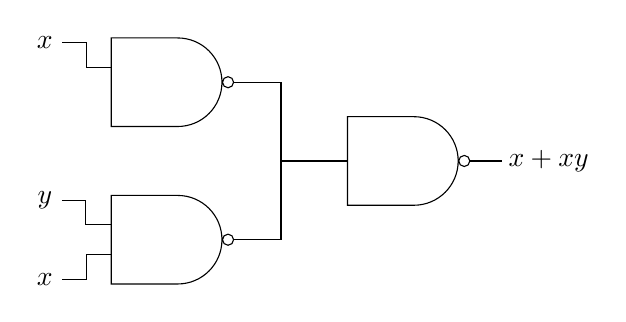
\begin{tikzpicture}[ circuit symbol wires]
    
    \node (x) at (0,0) {$x$};
    \node (y) at (0,1) {$y$};
    \node (z) at (0,3) {$x$};
    \node[nand gate US, minimum size=32pt, draw] at (1.5,0.5) (And) {};
    \node[nand gate US, minimum size=32pt, draw] at (1.5,2.5) (And1) {};
    \node[nand gate US, minimum size=32pt, draw] at (4.5,1.5) (And2) {};
    \draw (x.east) - ++(right:3mm) |- (And.input 2);
    \draw (y.east) - ++(right:3mm) |- (And.input 1);
    \draw (z.east) - ++(right:3mm) |- (And1.input 1);
    %\draw (y.east) - ++(right:3mm) |- (And1.input 2);
    \draw (3.85,1.5) -- (3,1.5);
    \draw (3,0.5) -- (3,2.5);
    \draw (And.output) -- ($(And) + (1.5,0)$);
    \draw (And1.output) -- ($(And) + (1.5,2)$);
    \node (z) at ($(And2) + (1.9,0)$) {$x+xy$};
    \draw (5.4,1.5) -- (5.8,1.5);
    
    \end{tikzpicture}
    \end{center}
\end{document}
